\documentclass[11pt]{article}
\usepackage{amssymb, latexsym, amsmath, verbatim, multicol, pdfpages}
\usepackage{hyperref} % Required for adding linksand customizing them
\urlstyle{same}
\definecolor{linkcolour}{rgb}{0,0.2,0.6} % Link color
\hypersetup{colorlinks,breaklinks,urlcolor=linkcolour,linkcolor=linkcolour}


\setlength{\oddsidemargin}{-.25in} \setlength{\evensidemargin}{-.25in} \setlength{\textwidth}{6.8in}
\setlength{\textheight}{9.3in} \setlength{\topmargin}{-.8in} \setlength\parindent{0pt}      

\newcommand{\fakesection}[1]{%
  \par\refstepcounter{section}% Increase section counter
  \sectionmark{#1}% Add section mark (header)
  \addcontentsline{toc}{section}{\protect\numberline{\thesection}#1}% Add section to ToC
  % Add more content here, if needed.
}

\newcommand{\fakesectionnocounter}[1]{%
  % \par\refstepcounter{section}% Increase section counter
  \sectionmark{#1}% Add section mark (header)
   \addcontentsline{toc}{section}{\protect\numberline{}#1}% Add section to ToC
  % Add more content here, if needed.
}

\begin{document}


\begin{center}
  {\Large Math 220-01: Mathematical Reasoning and Proof \\ Instructor: David Zureick-Brown (``DZB'')\smallskip}
\end{center}
\vskip-.05in

\vskip.25in
\begin{center}
 \noindent\textbf{``Notes''}\\
 Last updated: \today\\
\end{center}

These are very rough notes for the course, which mostly overlap with the class content.

\tableofcontents



 \expandafter\newcommand\csname topic1\endcsname{Introduction to course. Mathematical reasoning. Logic}
 \expandafter\newcommand\csname topic2\endcsname{``Direct" proofs, proof by ``cases'' and divisibility problems}
 \expandafter\newcommand\csname topic3\endcsname{Proof by contradiction}
 \expandafter\newcommand\csname topic4\endcsname{Induction}
 \expandafter\newcommand\csname topic5\endcsname{Set theory. Basic operations. Proofs with sets} 
 \expandafter\newcommand\csname topic6\endcsname{More sets. DeMorgan’s laws. Cartesian Products. Power sets}
 \expandafter\newcommand\csname topic7\endcsname{Introduction to functions; images and surjectivity}
 \expandafter\newcommand\csname topic8\endcsname{Inverse Image (or “Preimage”)}
 \expandafter\newcommand\csname topic9\endcsname{Injectivity}
 \expandafter\newcommand\csname topic10\endcsname{Composition of functions}
 \expandafter\newcommand\csname topic11\endcsname{Inverse functions}
 \expandafter\newcommand\csname topic12\endcsname{Relations}
 \expandafter\newcommand\csname topic13\endcsname{(Un)countability}

\newpage

\fakesection{\csname topic1\endcsname}  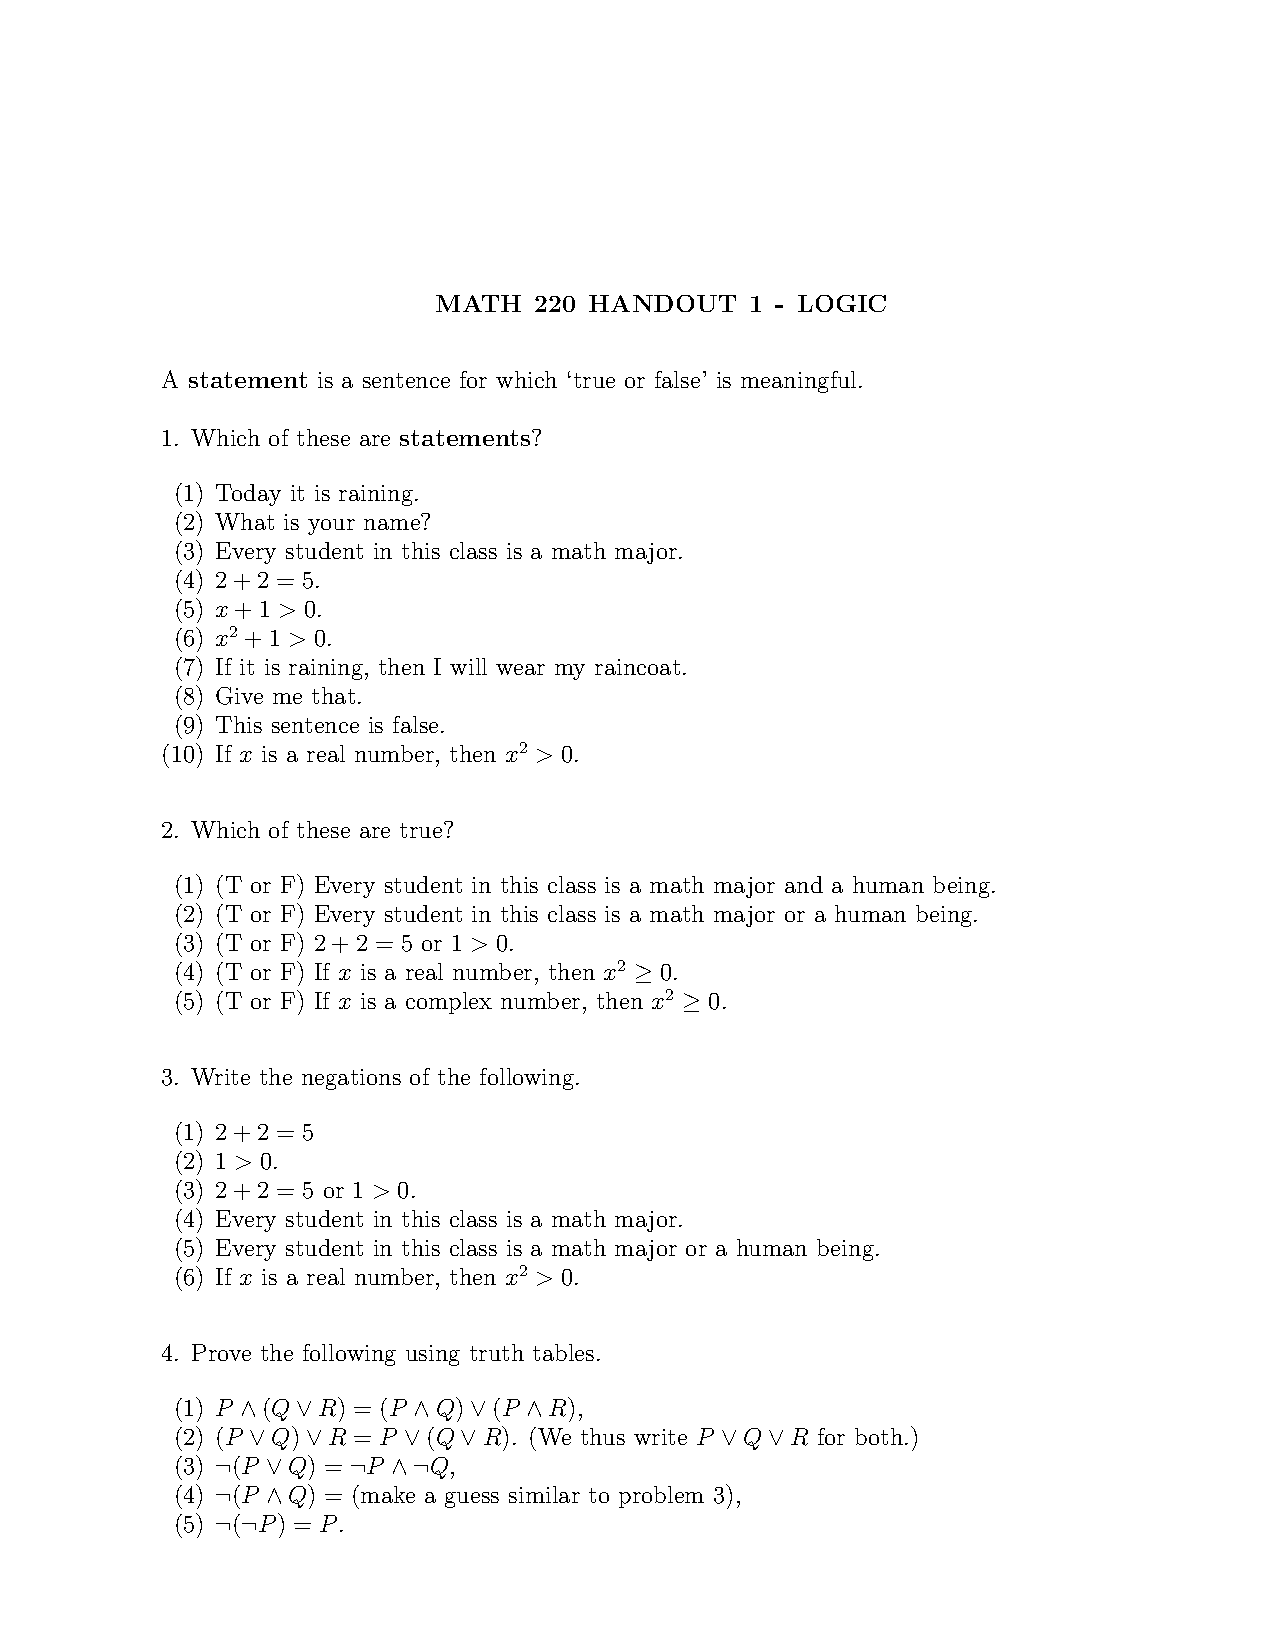
\includepdf[pages=-]{DZB-notes/220-01-logic}
\fakesection{\csname topic2\endcsname}  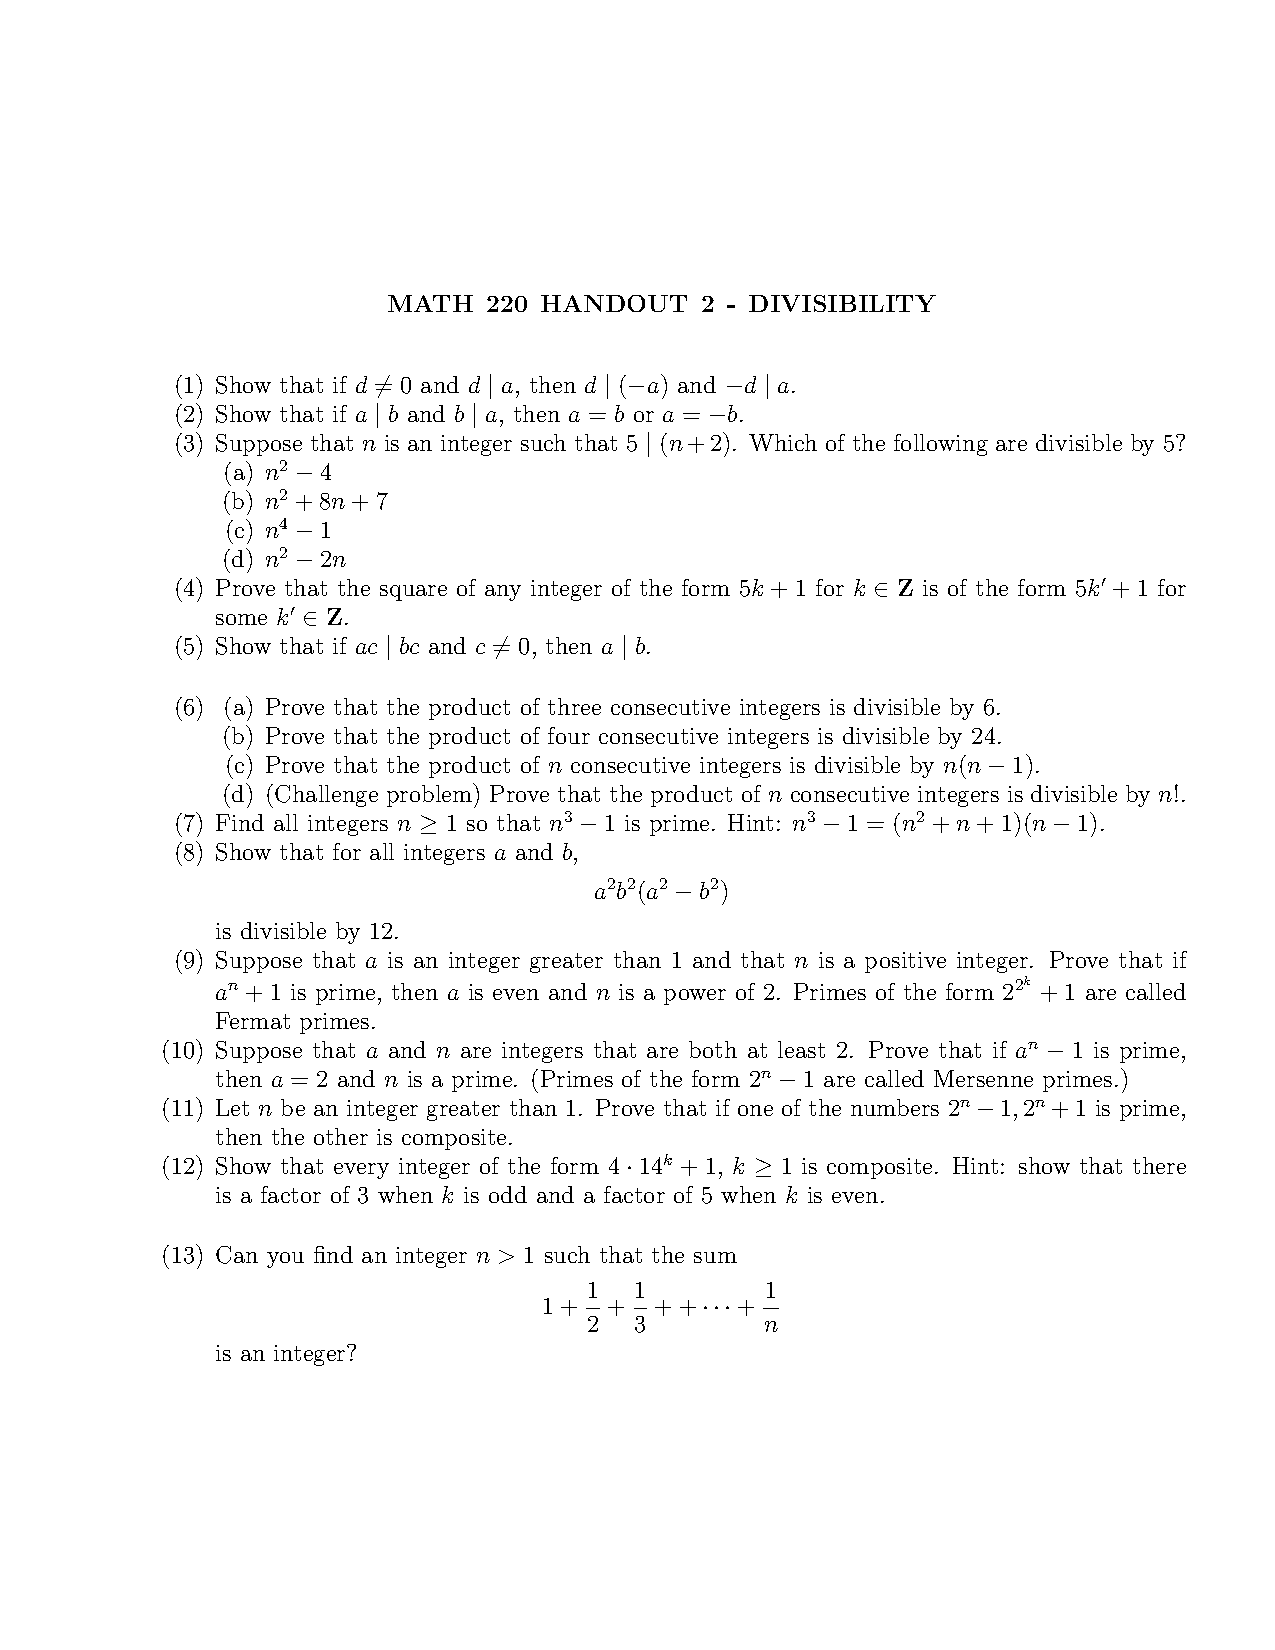
\includepdf[pages=-]{DZB-notes/220-02-divisibility}
\fakesection{\csname topic3\endcsname}  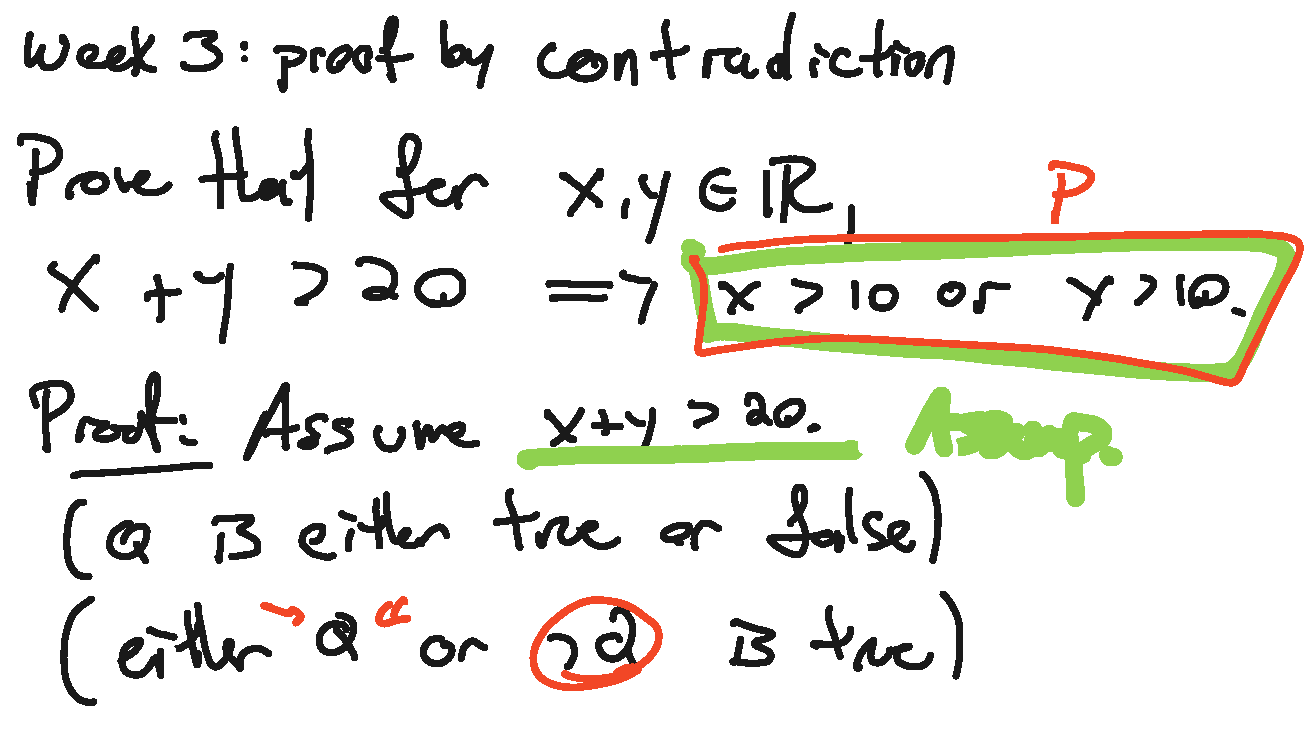
\includepdf[pages=-]{DZB-notes/220-03-contradiction-1}
                                        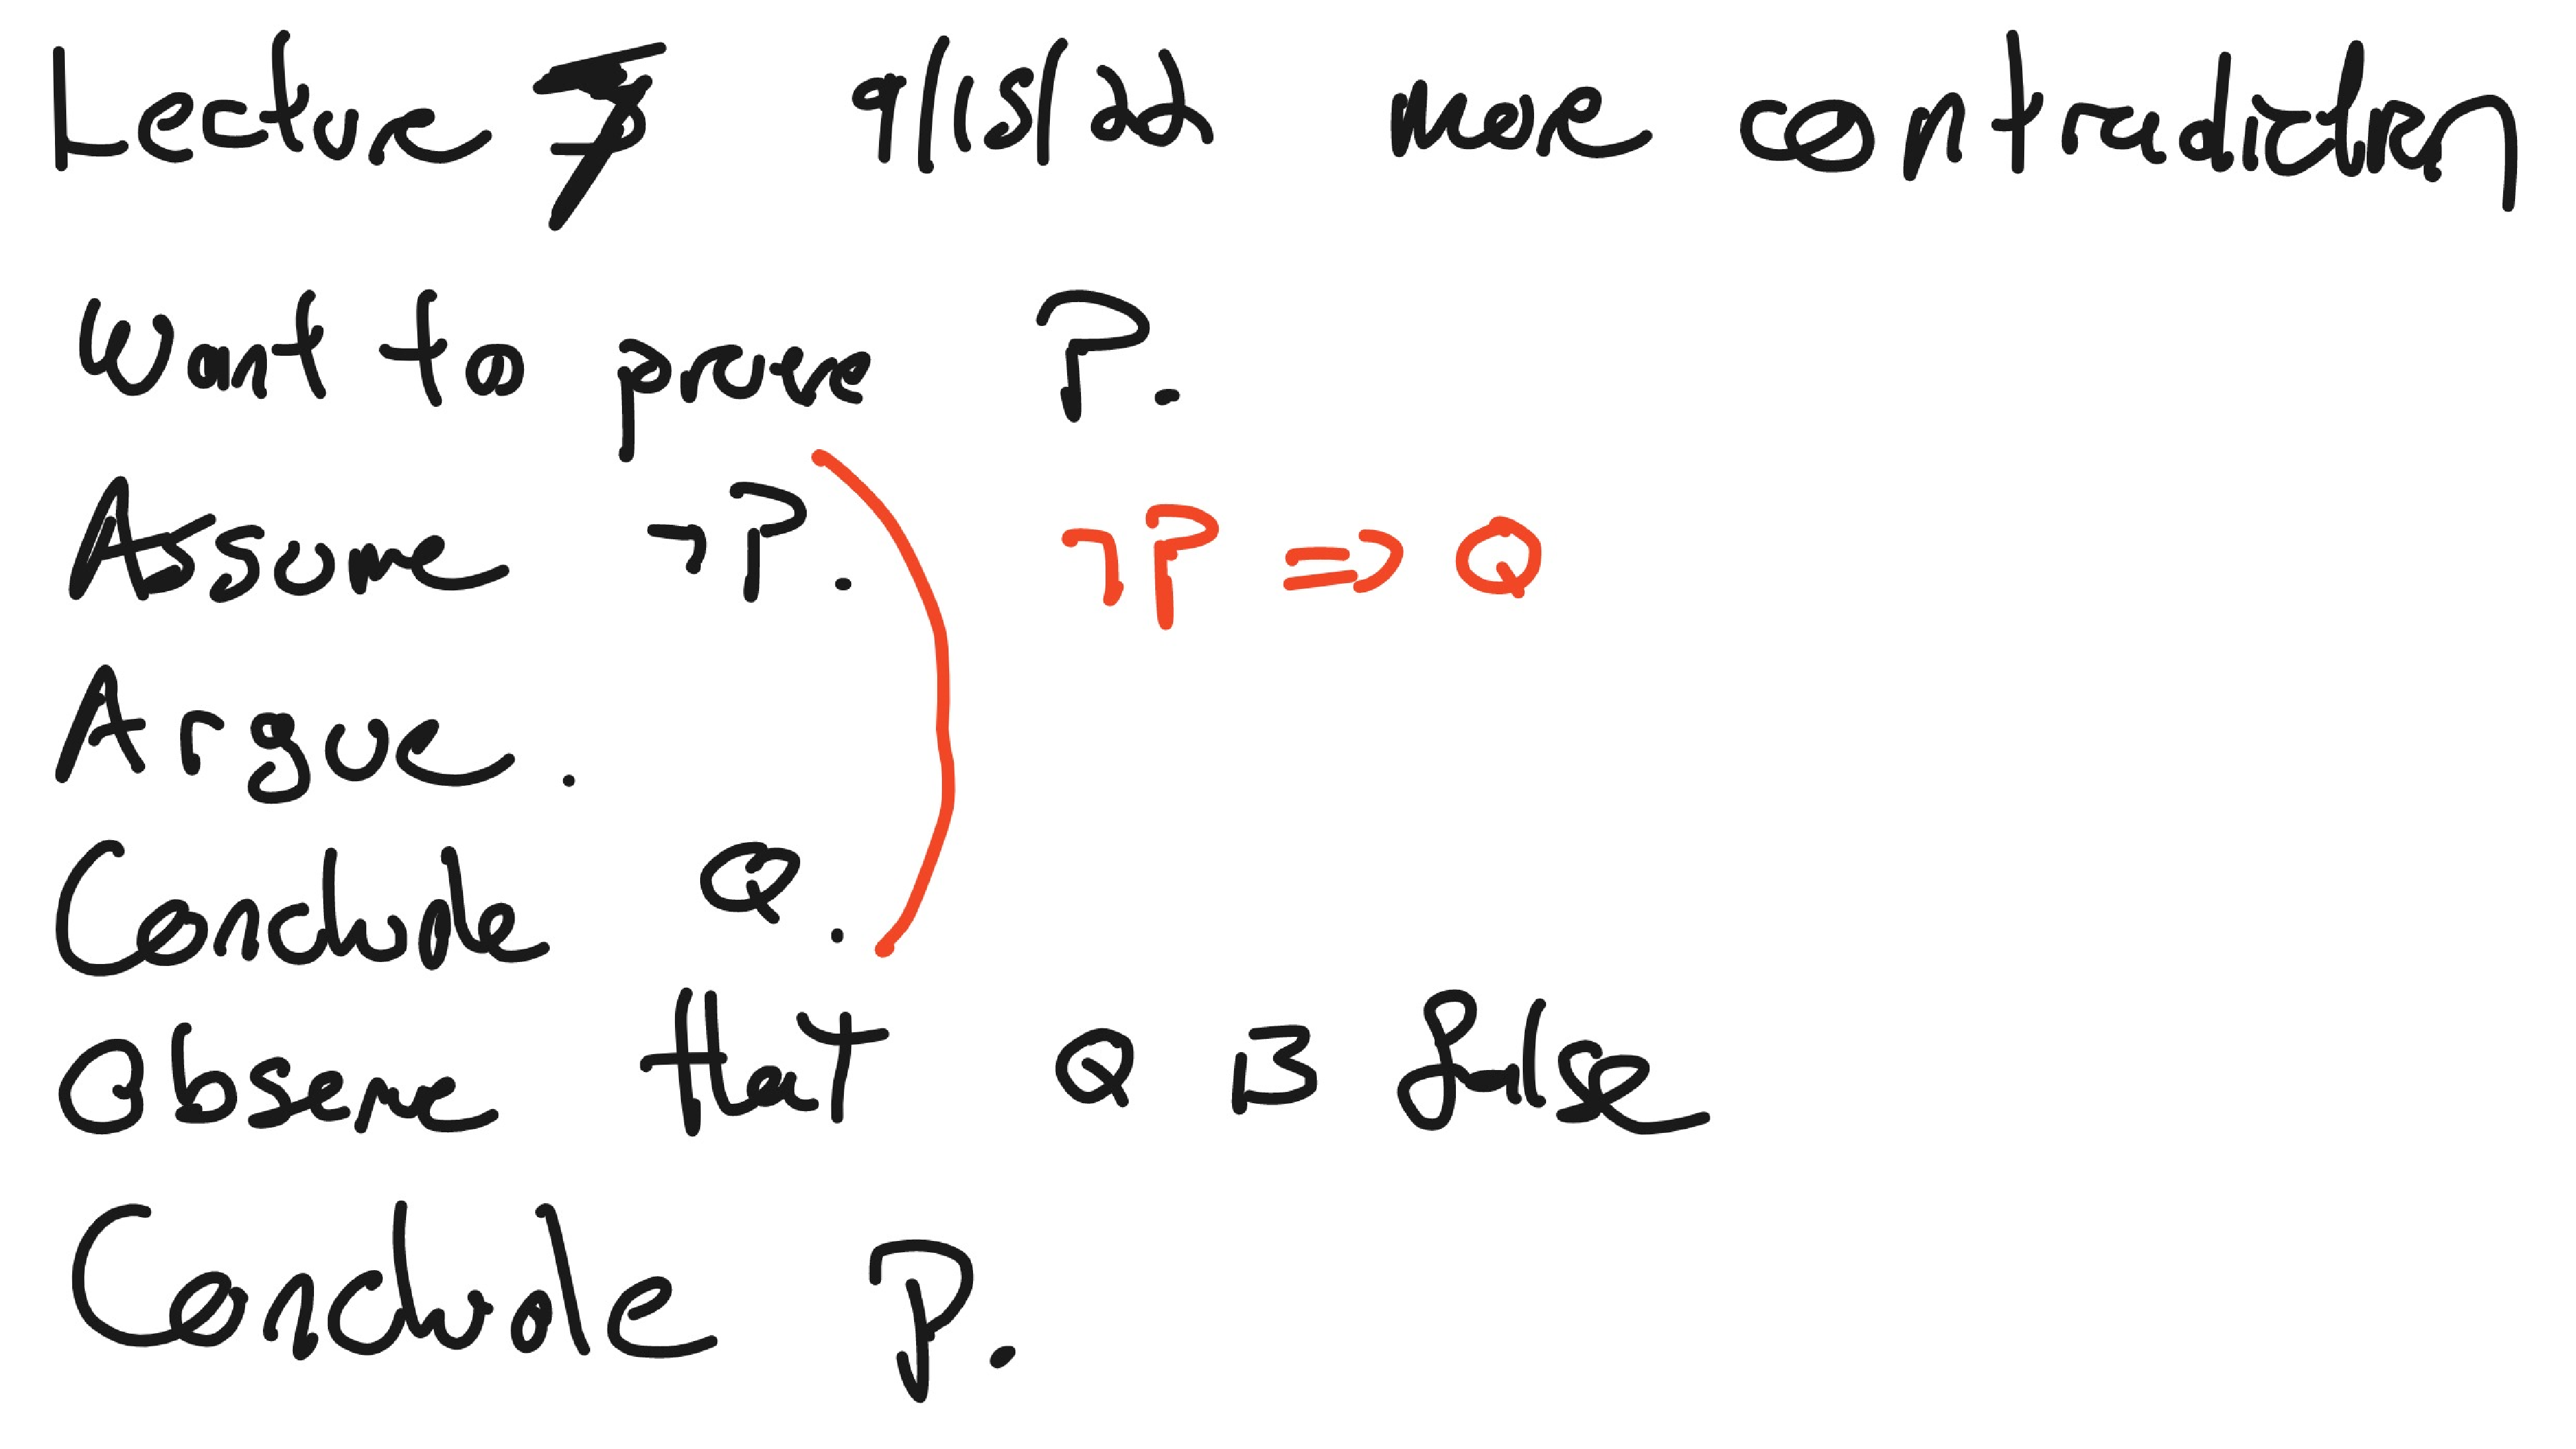
\includepdf[pages=-]{DZB-notes/220-03-contradiction-2}
\fakesection{\csname topic4\endcsname}  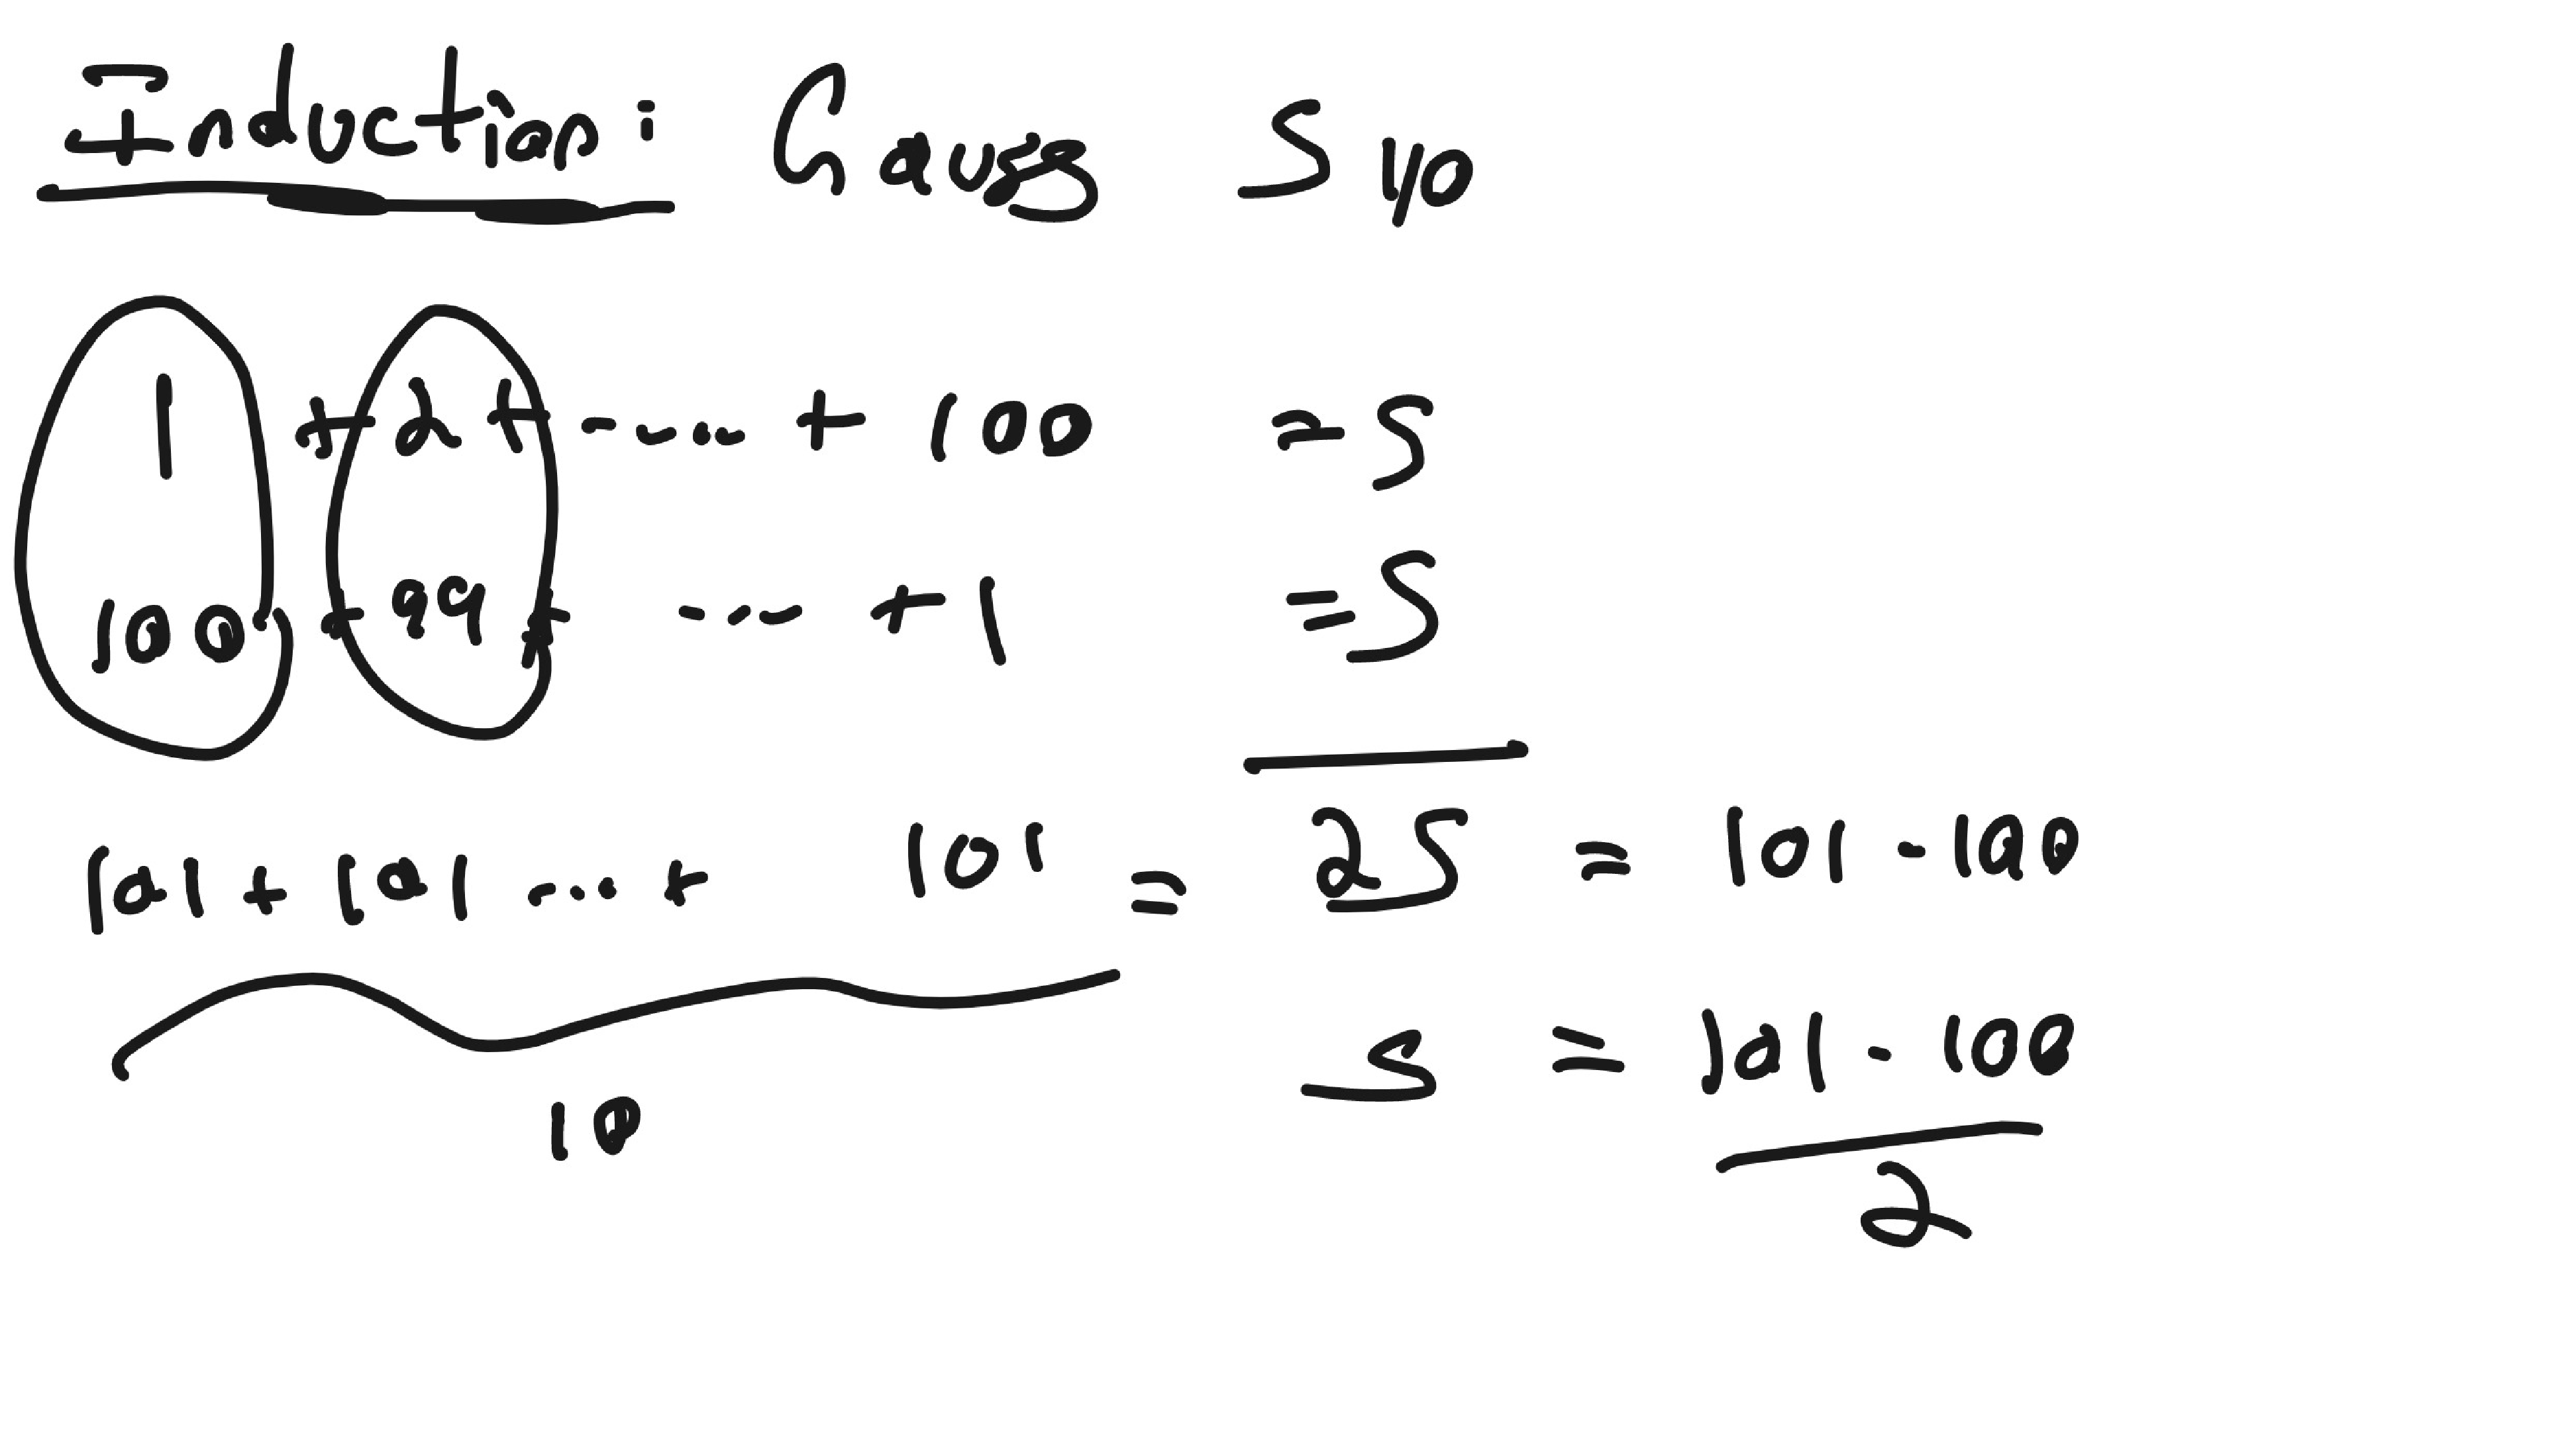
\includepdf[pages=-]{DZB-notes/220-04-induction-1}
                                        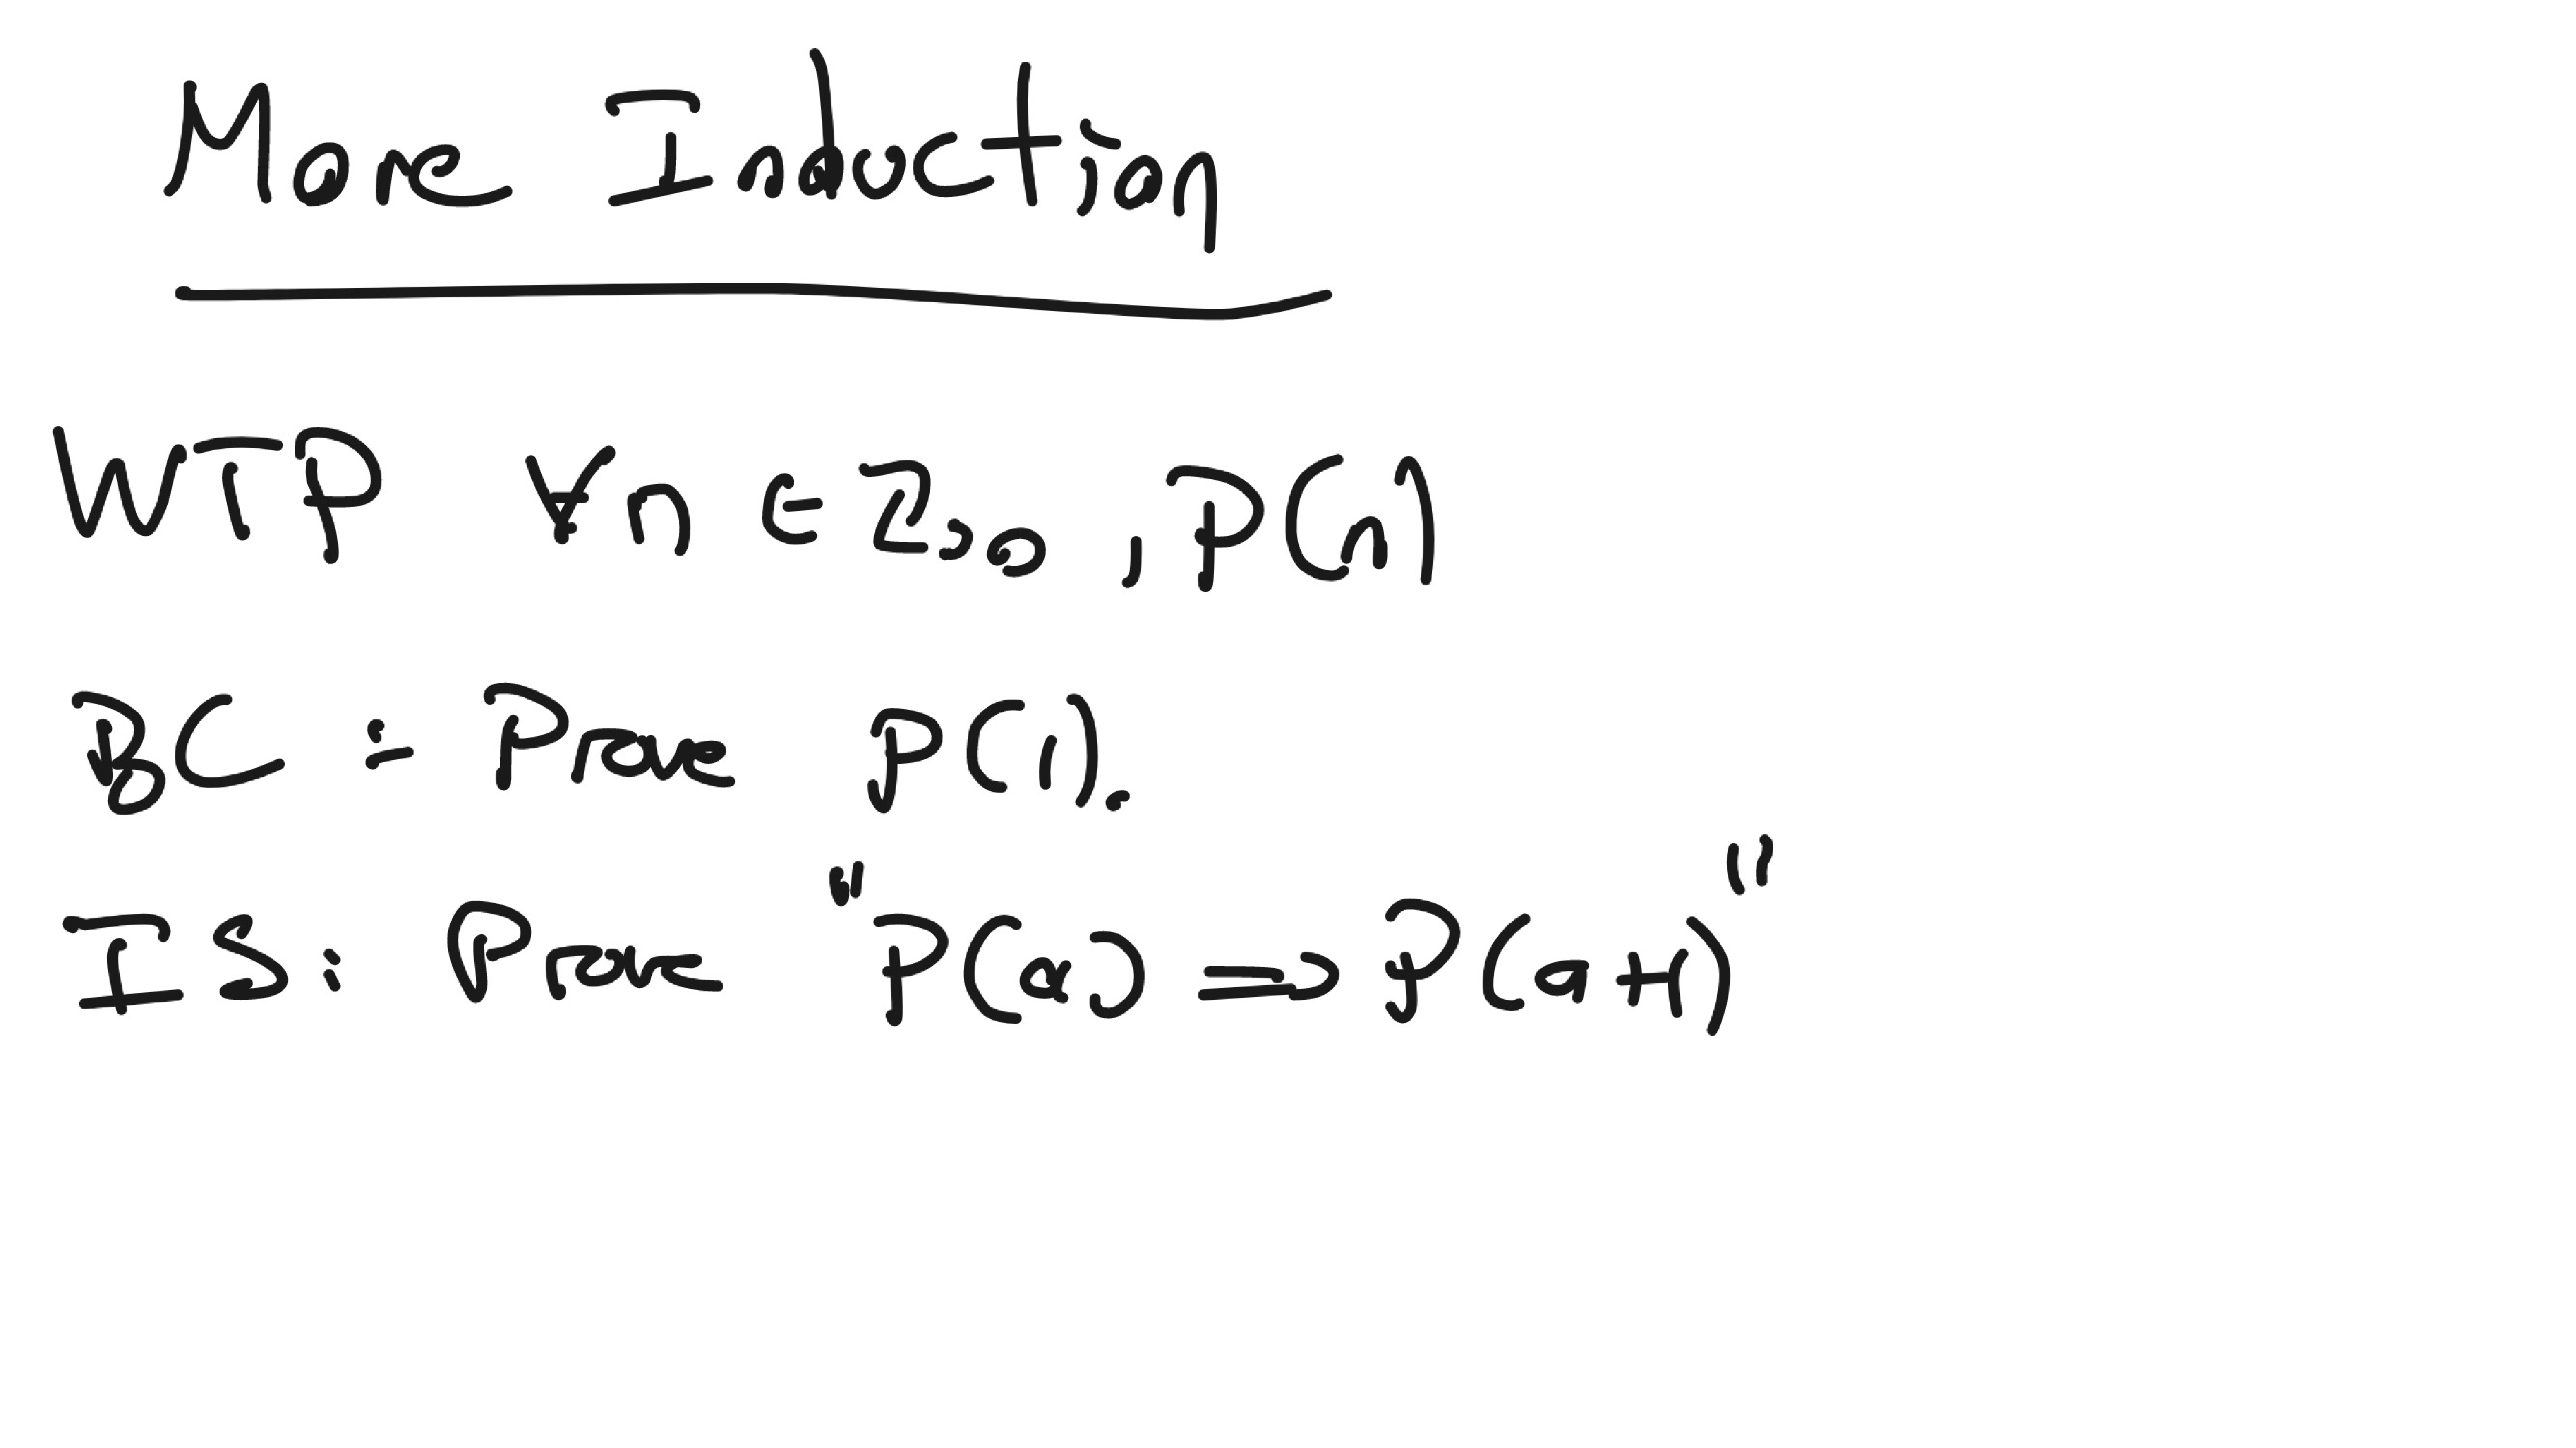
\includepdf[pages=-]{DZB-notes/220-04-induction-2}
\fakesection{\csname topic5\endcsname}  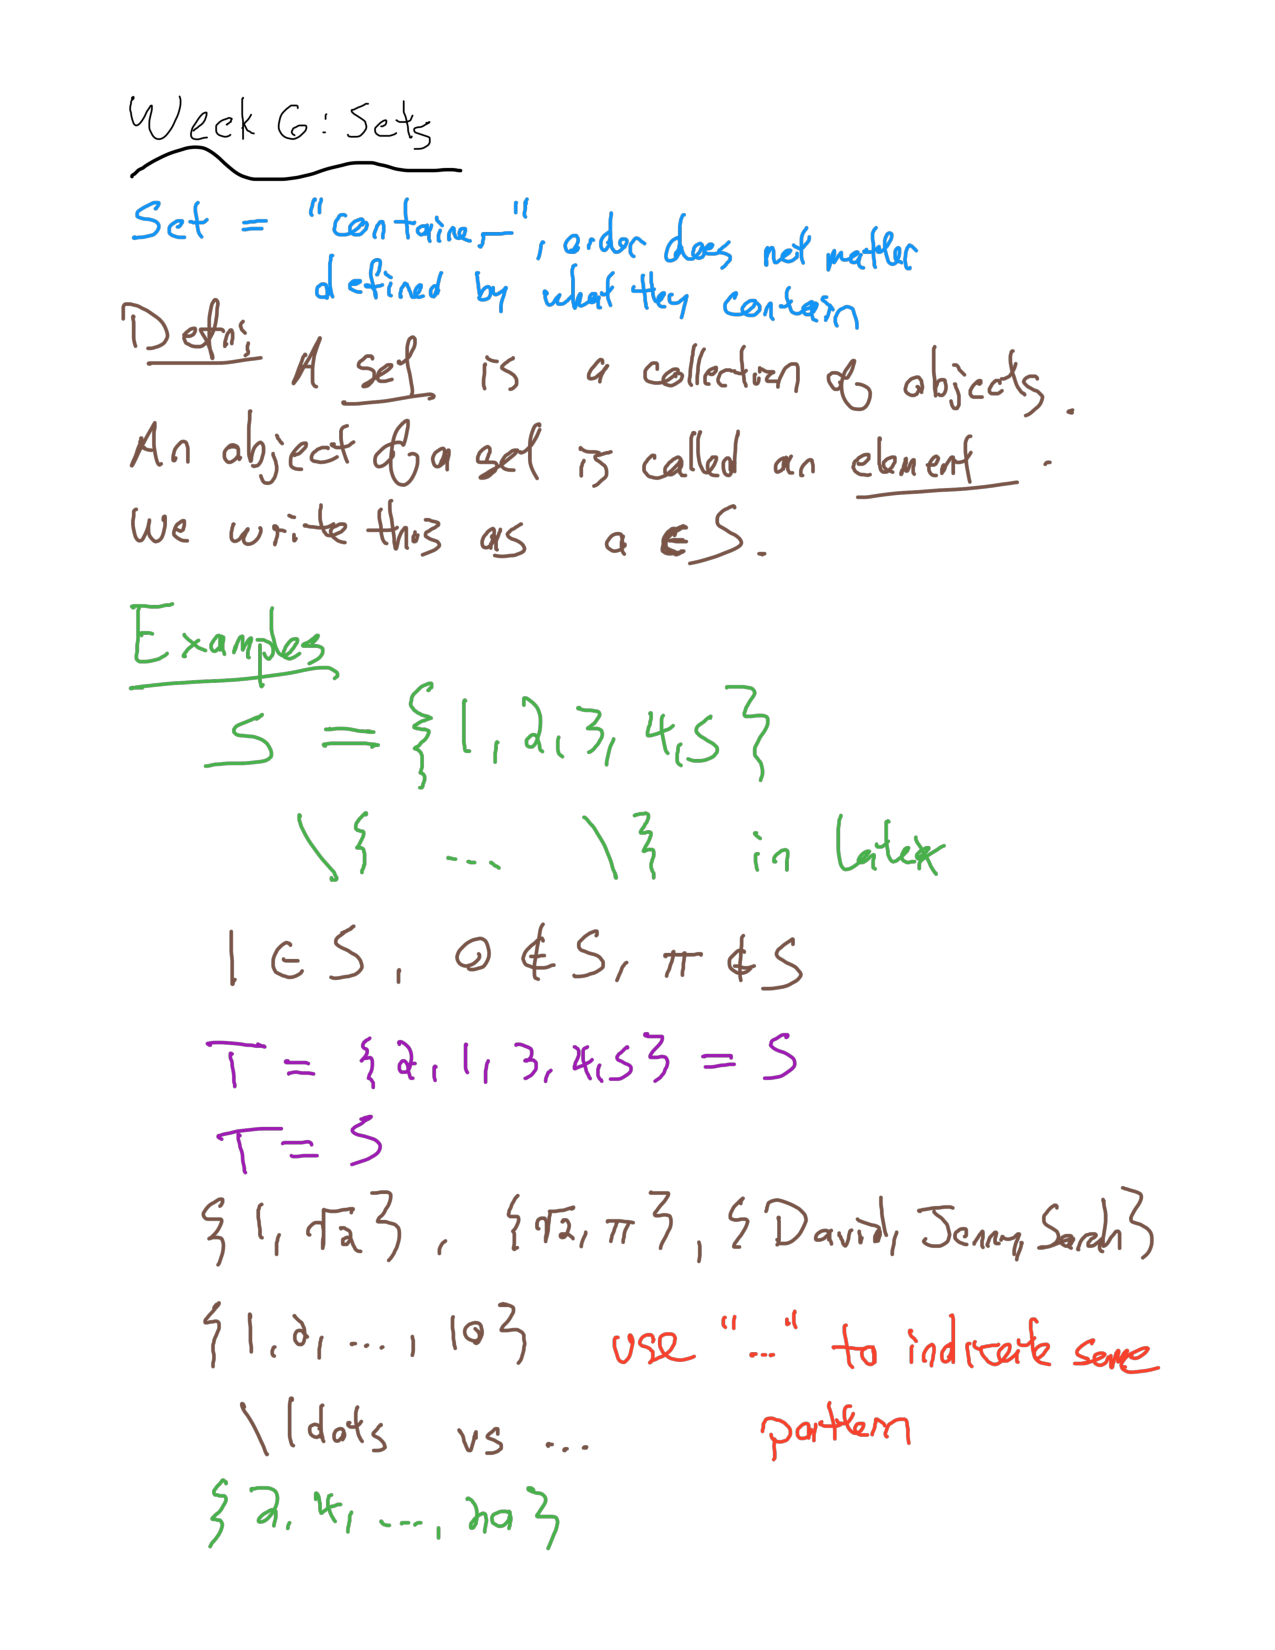
\includepdf[pages=-]{DZB-notes/220-05-whiteboard-sets}
\fakesection{\csname topic6\endcsname}  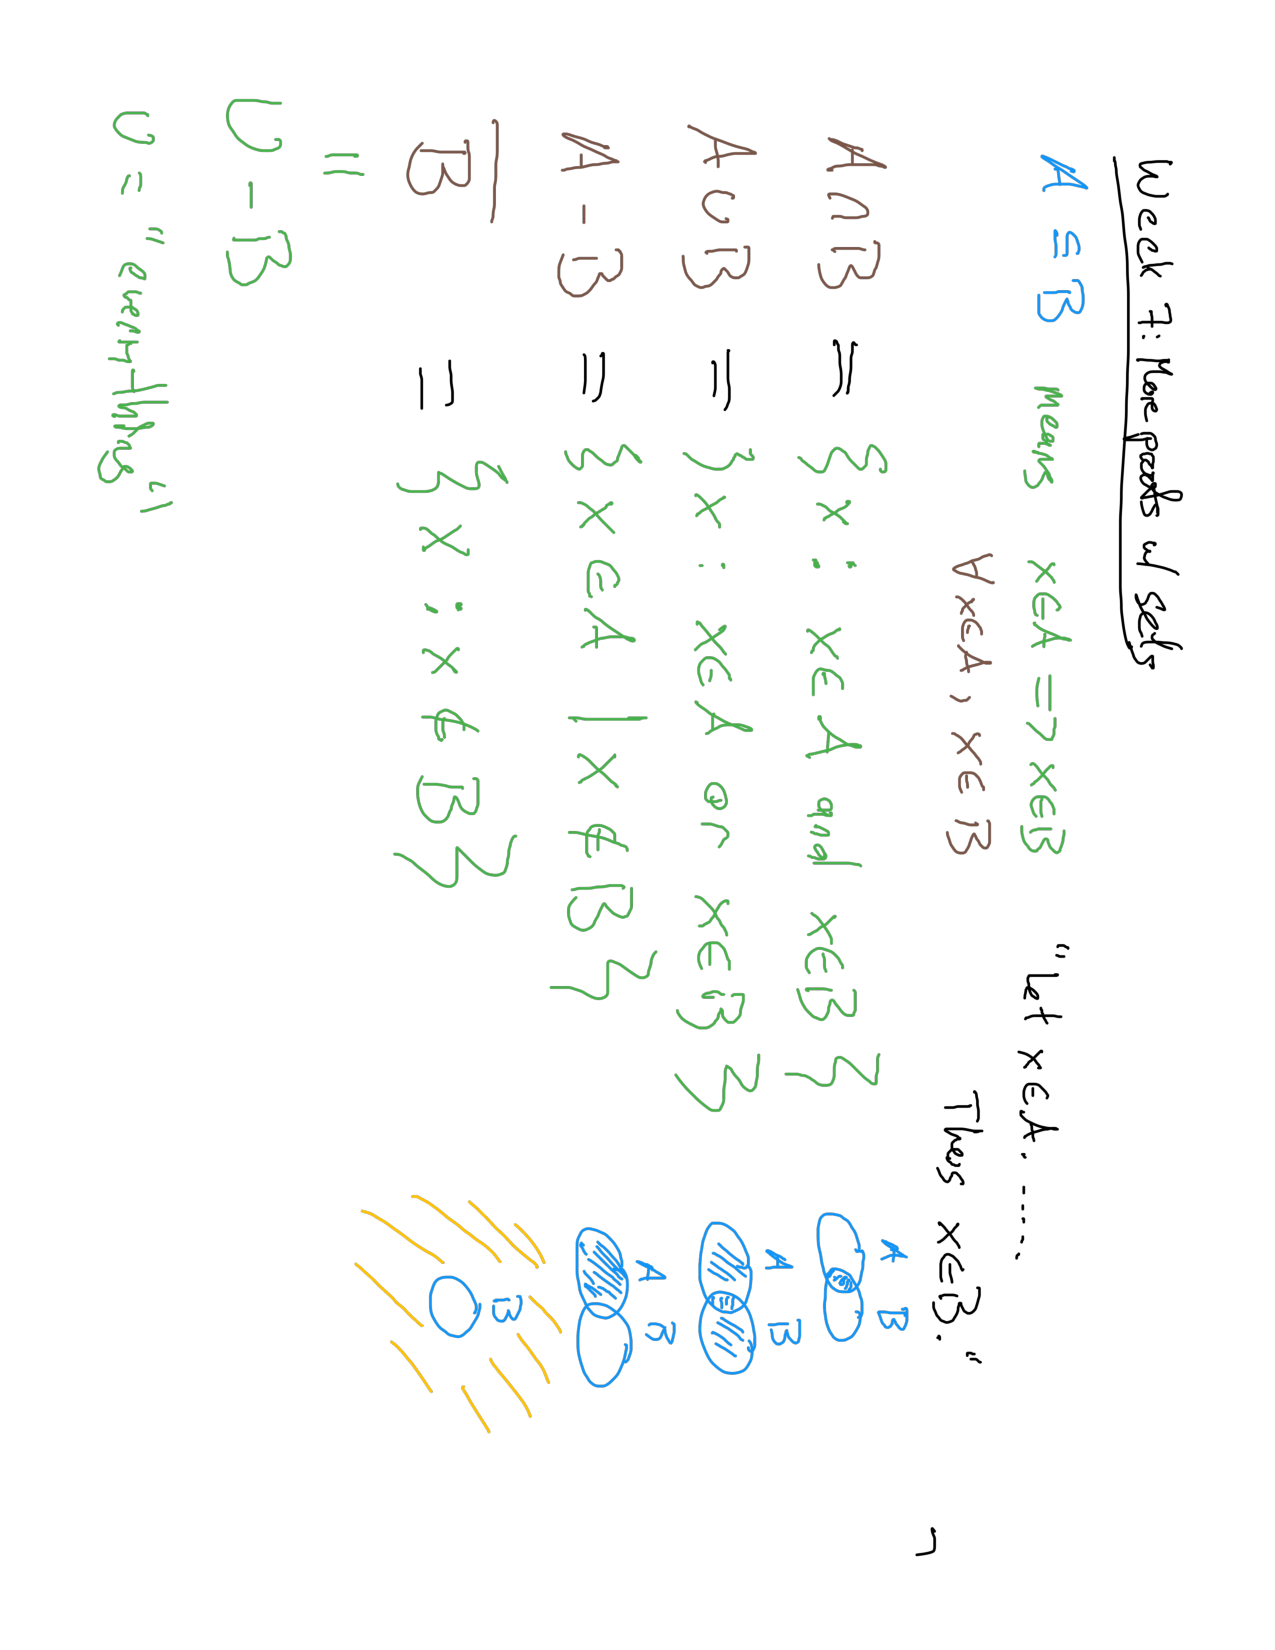
\includepdf[pages=-]{DZB-notes/220-06-whiteboard-more-sets}
\fakesection{\csname topic7\endcsname}  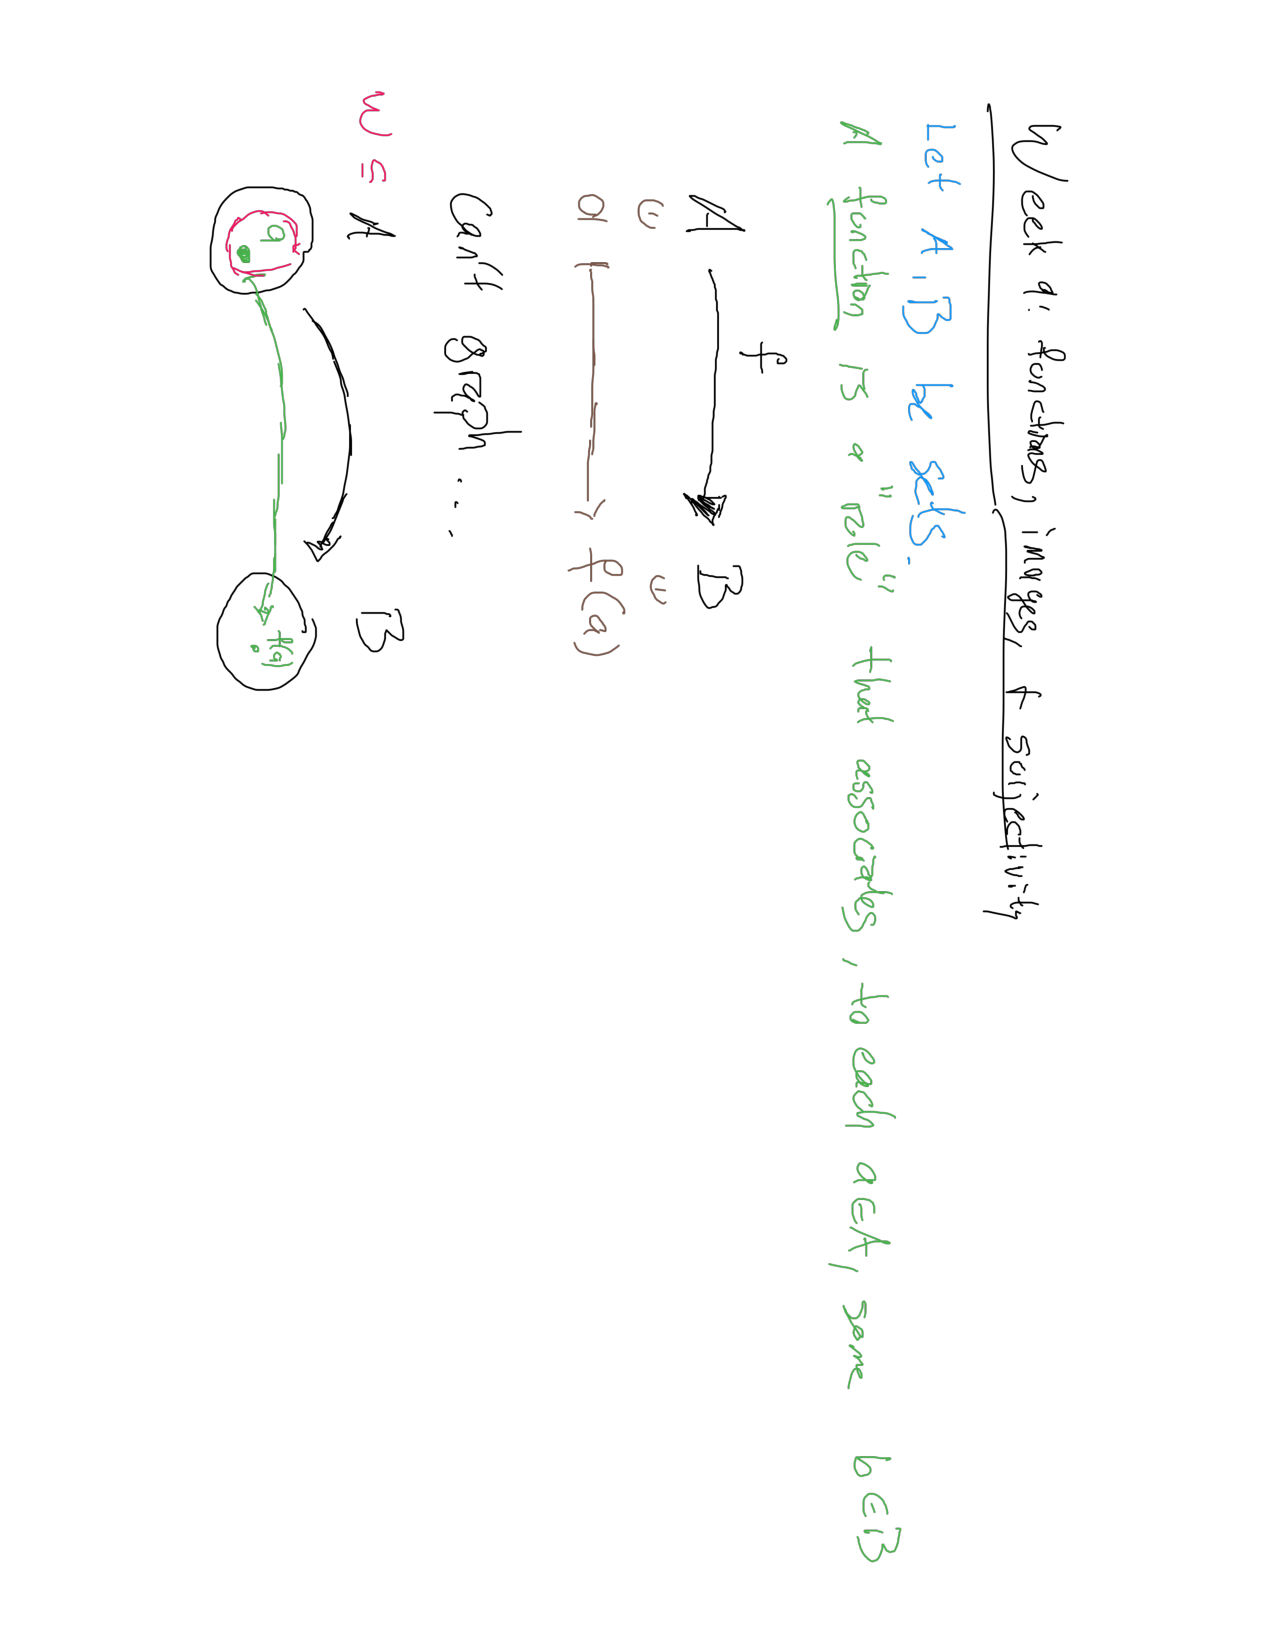
\includepdf[pages=-]{DZB-notes/220-07-whiteboard-functions}
\fakesection{\csname topic8\endcsname}  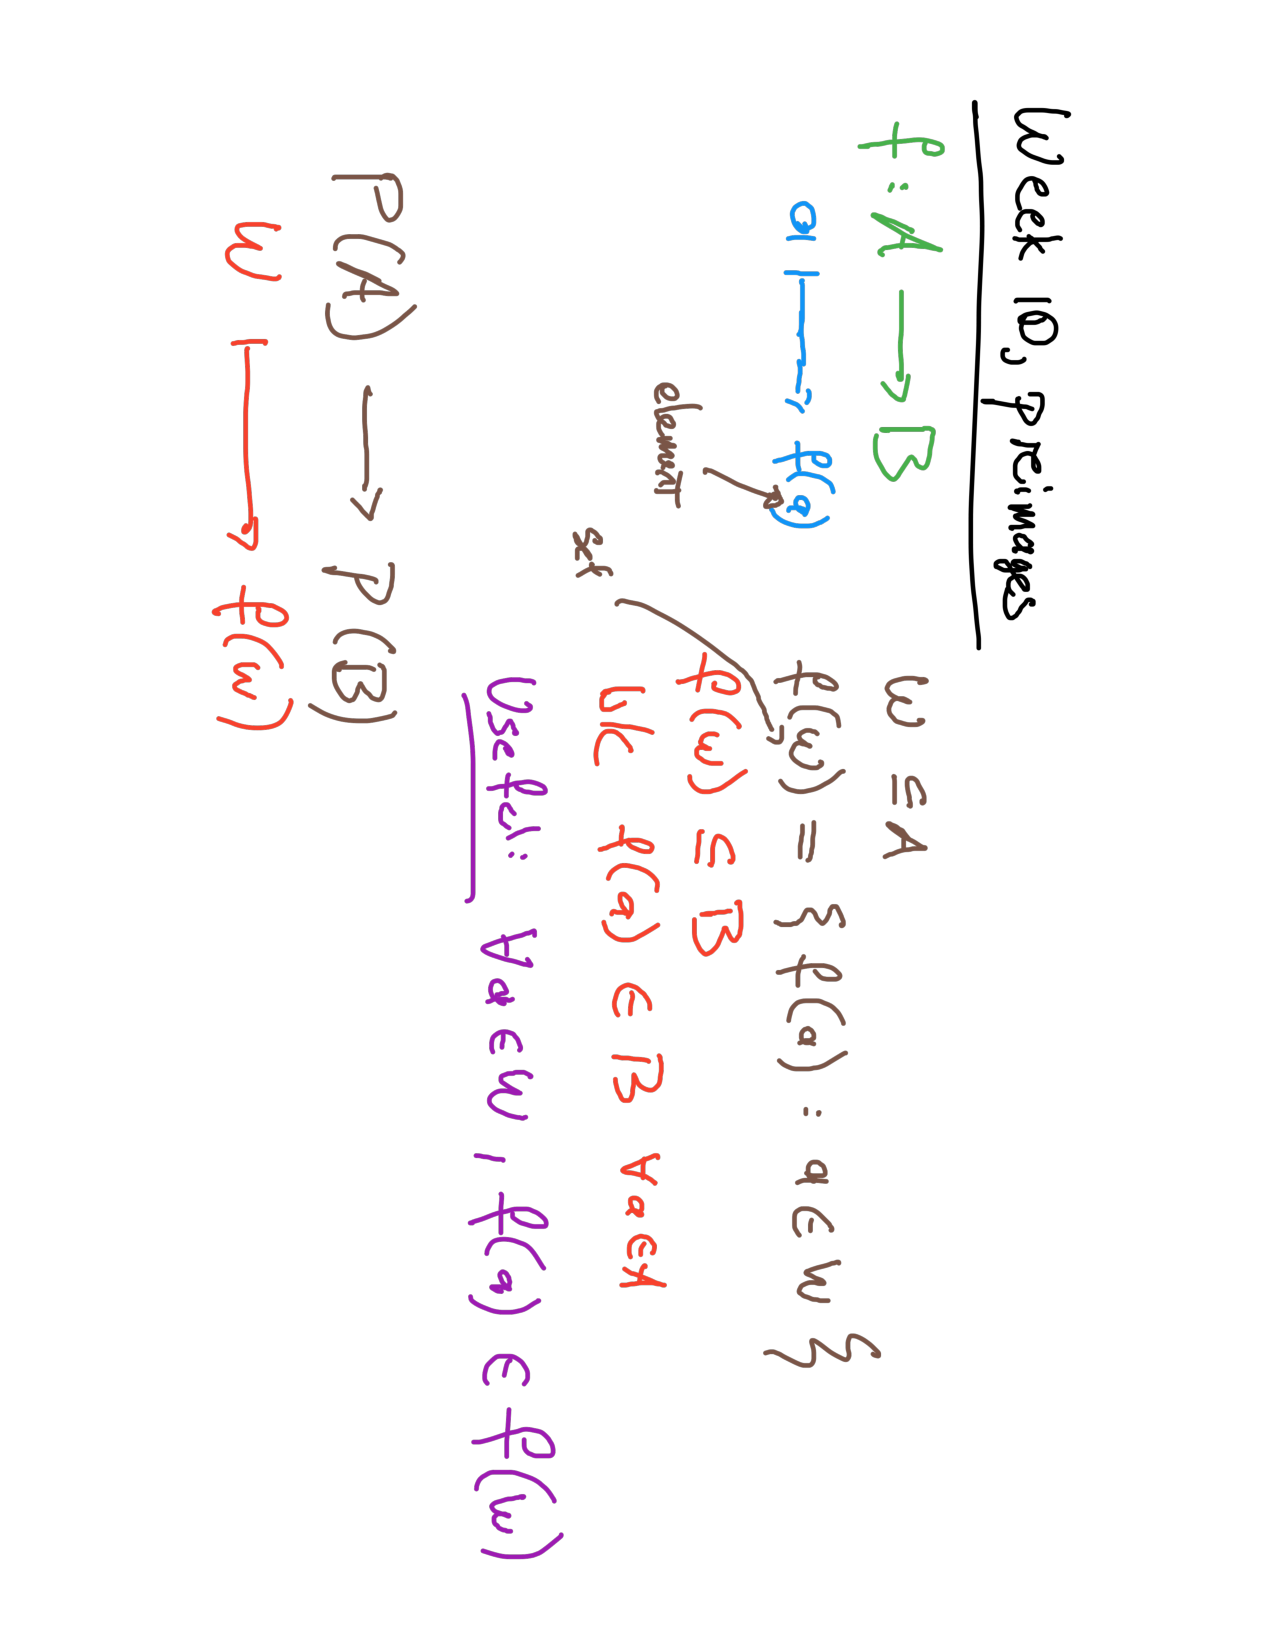
\includepdf[pages=-]{DZB-notes/220-08-whiteboard-preimages}
\fakesection{\csname topic9\endcsname}  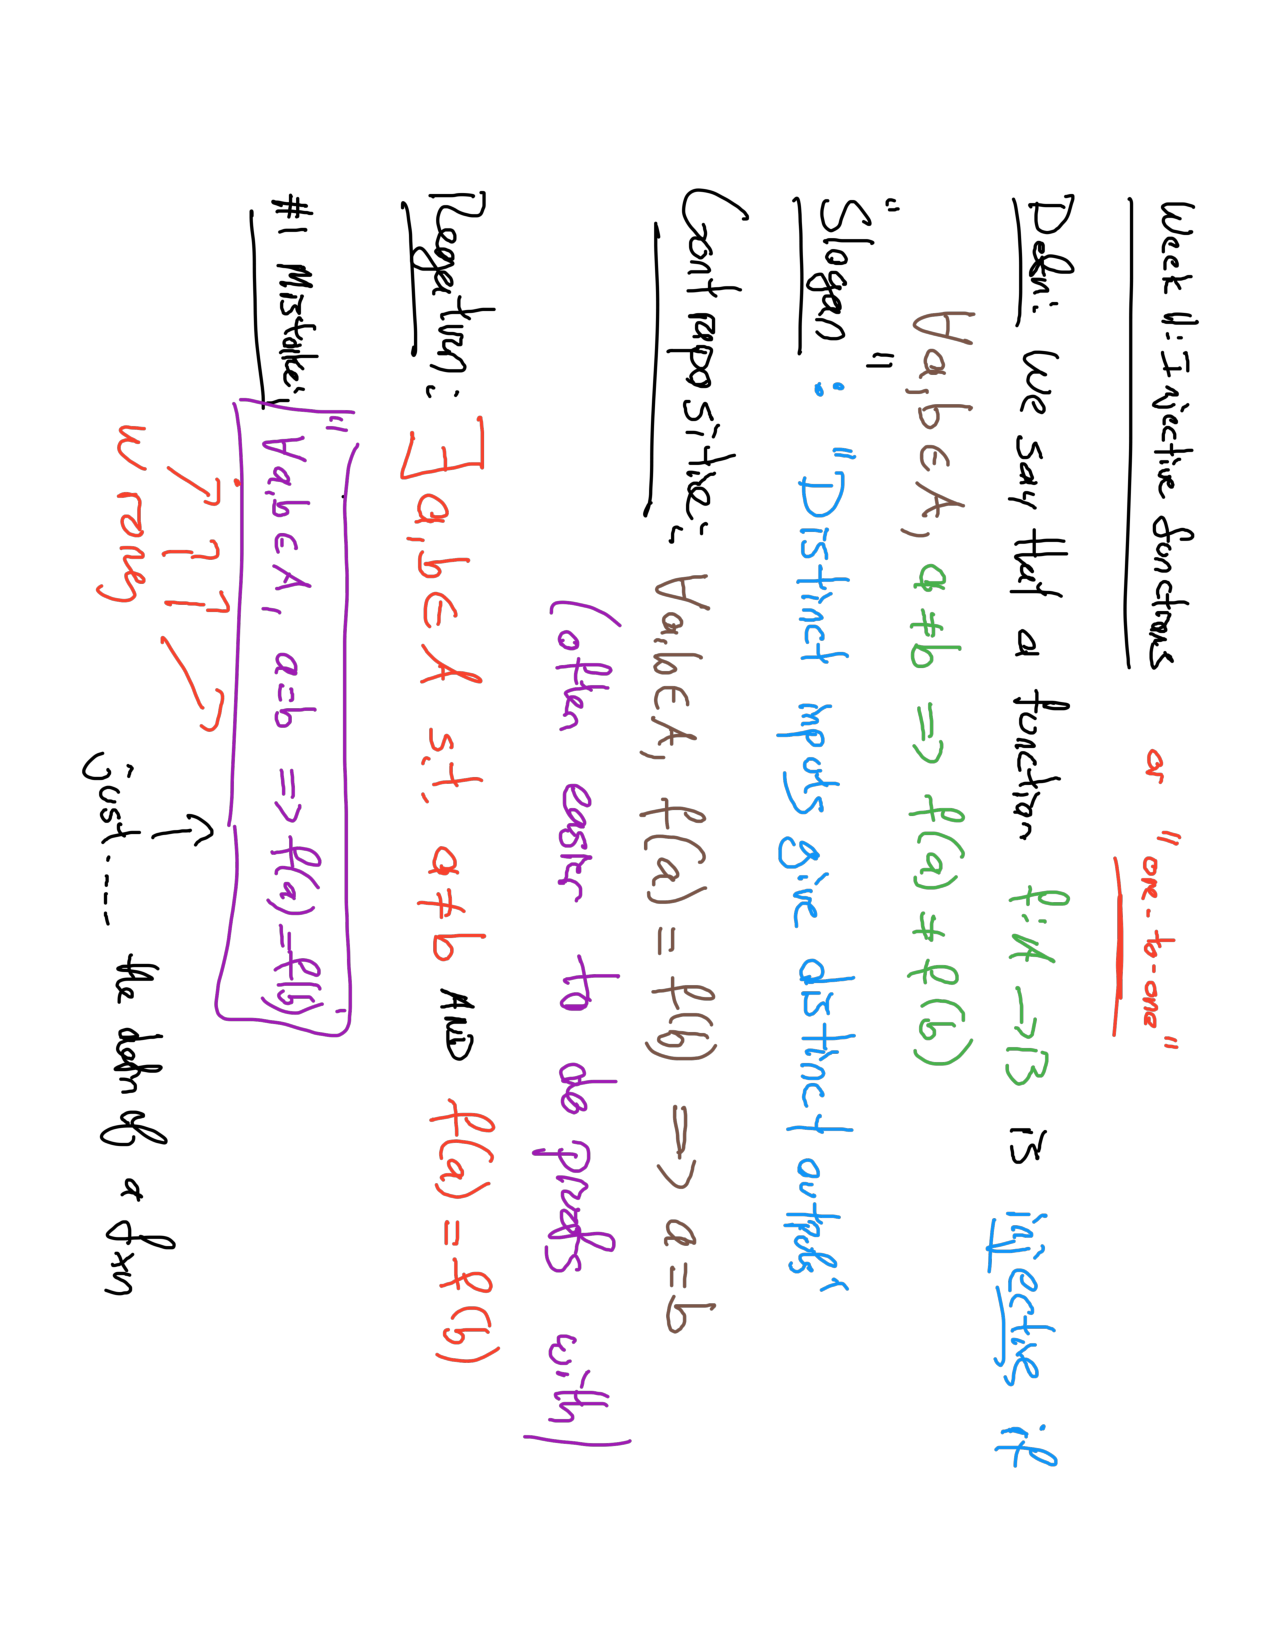
\includepdf[pages=-]{DZB-notes/220-09-whiteboard-injectivity}
\fakesection{\csname topic10\endcsname} 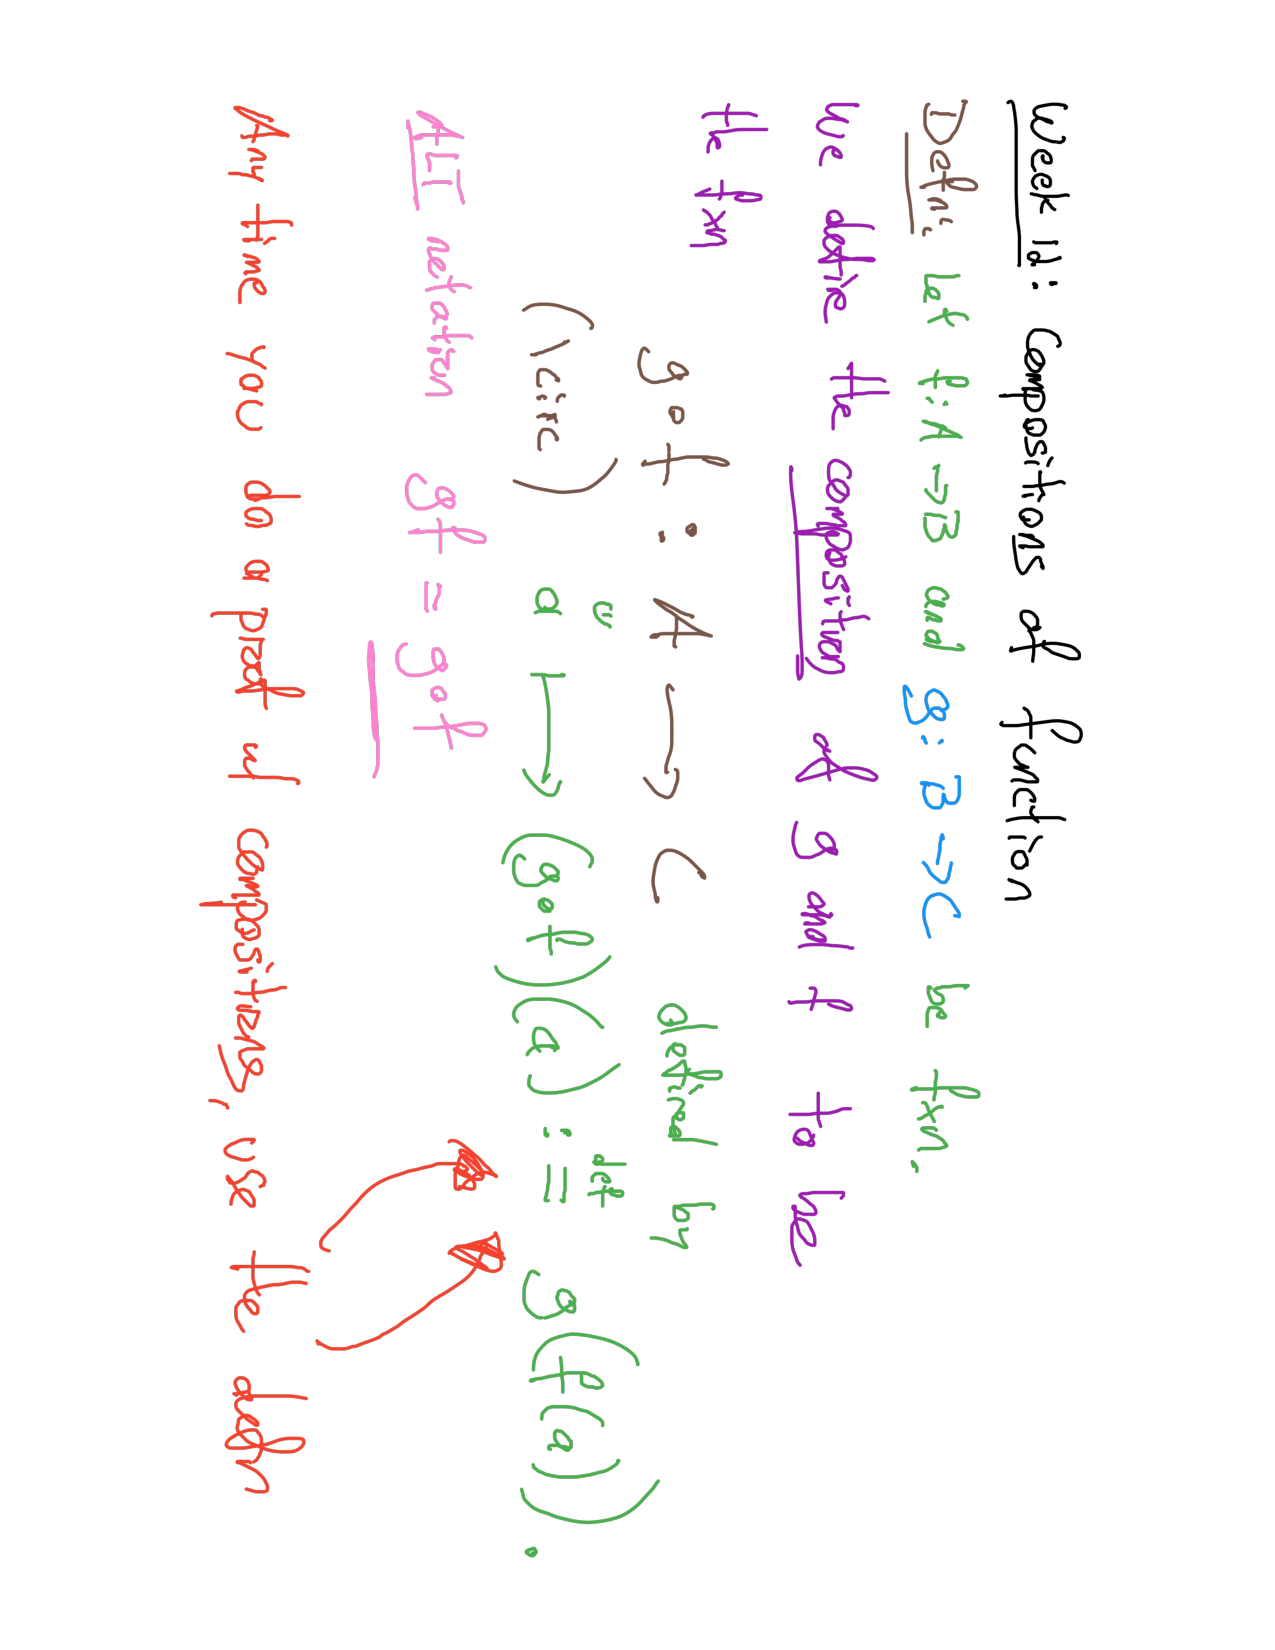
\includepdf[pages=-]{DZB-notes/220-10-whiteboard-composition}
\fakesection{\csname topic11\endcsname} 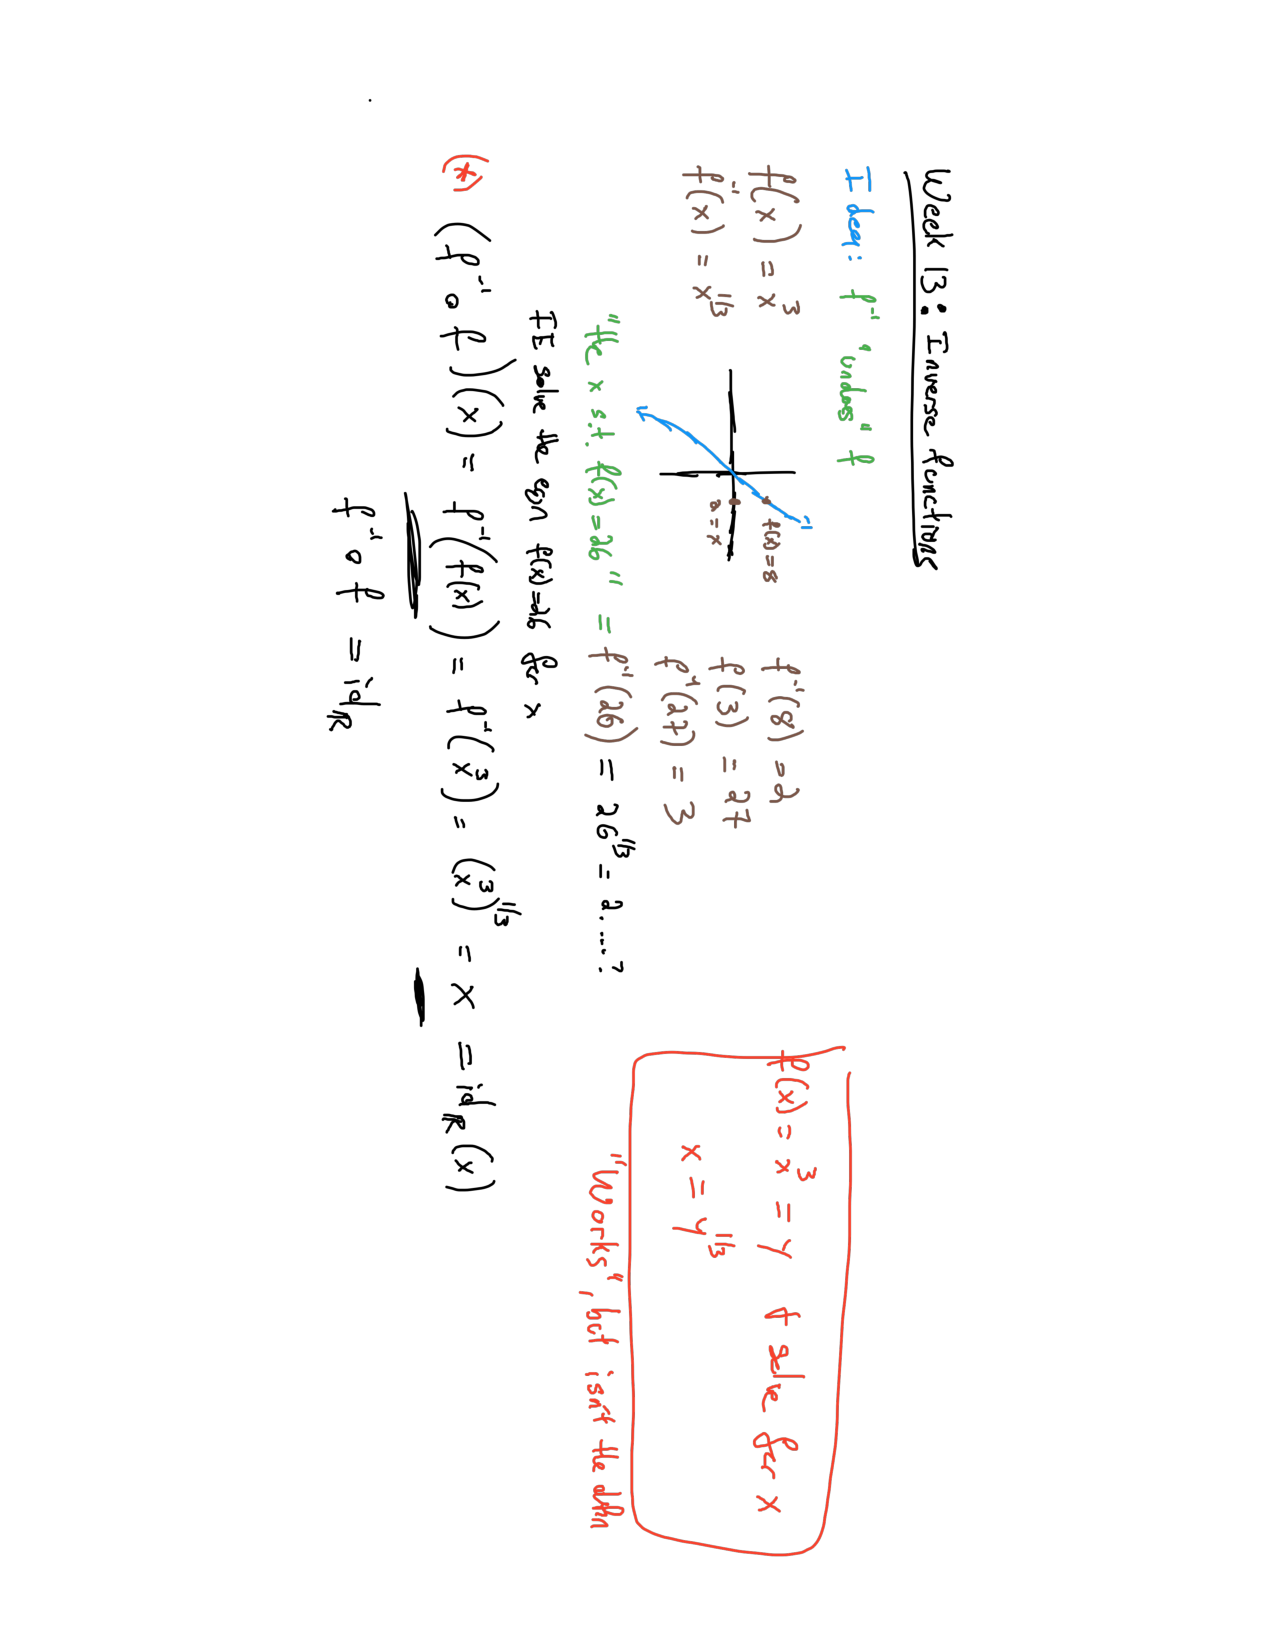
\includepdf[pages=-]{DZB-notes/220-11-whiteboard-inverses}
\fakesection{\csname topic12\endcsname} 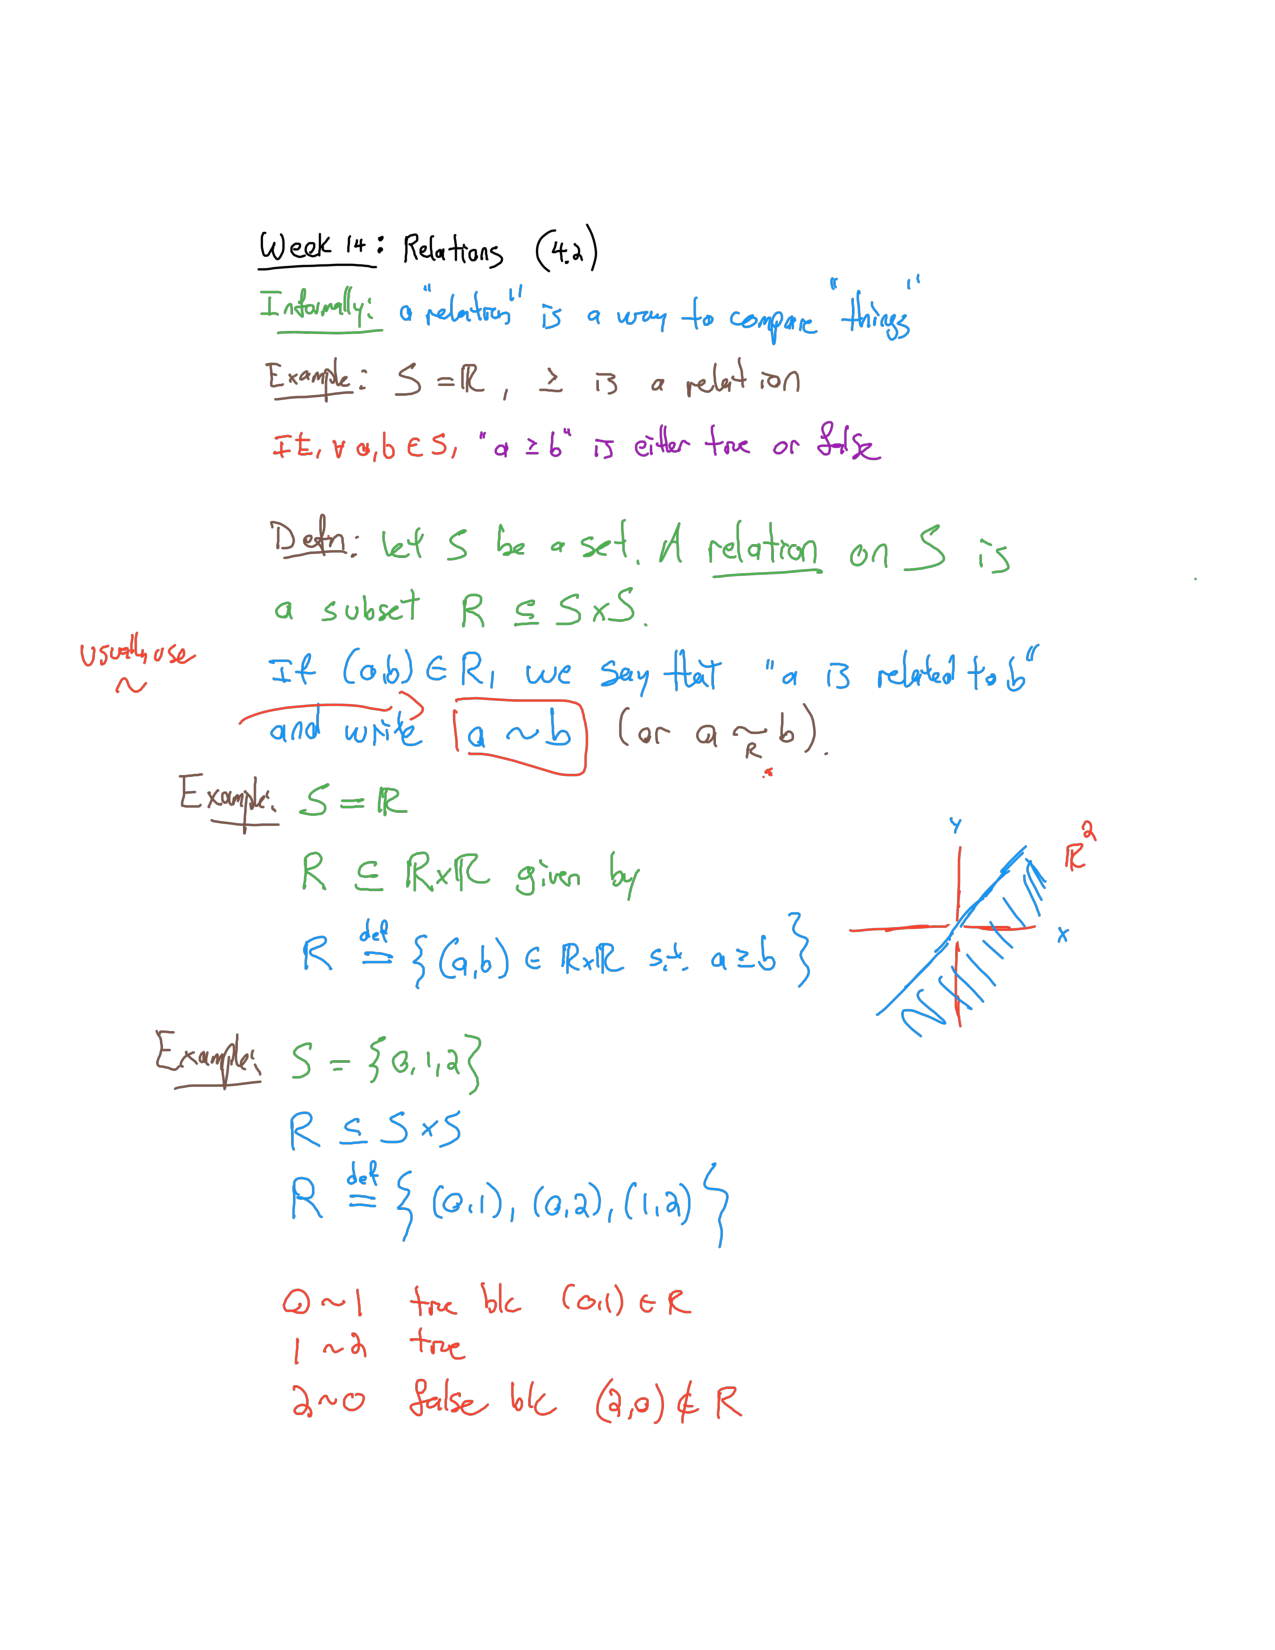
\includepdf[pages=-]{DZB-notes/220-12-whiteboard-relations}
% \fakesection{\csname topic13\endcsname} 

\end{document}

